%Appendeix2

%Not really sure what this pdf is, but I like it, and will post the link so I don't forget about it https://spie.org/samples/TT69.pdf
\section{Fluorescent Confocal Microscopy}
Confocal Microscopy is a technique capable of probing a sample with true 3-Dimensional optical resolution. The technique works by only allowing in focus light through a pinhole. By changing the plane of focus, one can traverse an object azimuthally or reconstruct a full three-dimensional image by compiling a ``stack'' of these images.  

\begin{wrapfigure}{r}{.5\textwidth}
	
	\centering
	\vspace{-1.2em}
	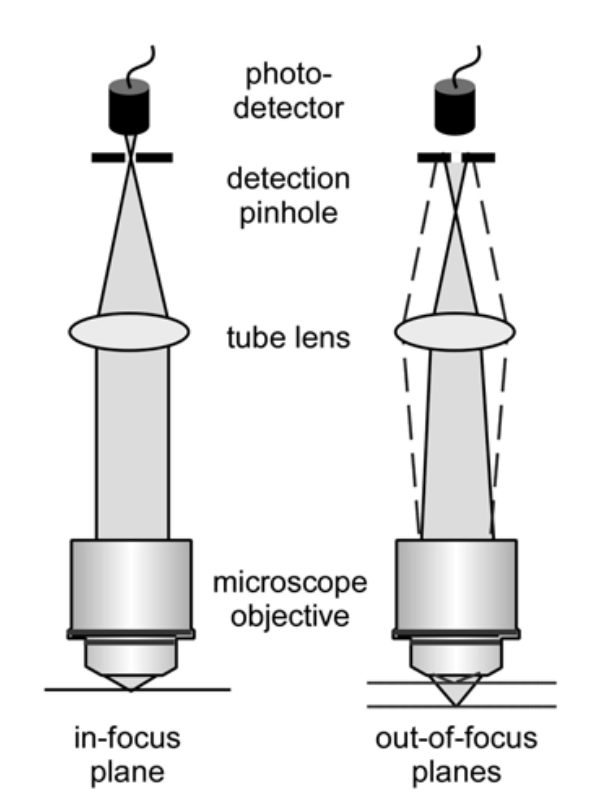
\includegraphics[width=\linewidth]{confocal_stuff/confocal_orig_fi_1-1}
	\caption[Confocal Optics 1]{PLACE HOLDER.}
	\label{fig:confocal_1}
	
	
\end{wrapfigure}
	
Fluorescent Confocal Microscopy works by the same general principle, only with the added complexity of optically-excitable fluorophores. These fluorophores absorb light from a narrow range of frequencies and re-emmit fluorescent light at a different known and specific frequency, which can then be measured. This allows for a greater resolution to larger objects, as well as the ability to detect objects that would otherwise be invisible to the microscope.  

Fluorescent Confocal Microscopy works by illuminating the specimen with a laser. The laser light passes through a pinhole, then is reflected by the dichroic mirror and then focused by the objective lens on a small area of the specimen. The re-emitted light from the fluorophores has a longer wavelength than the laser, so it is then transmitted through mirror.  It then then passes through the pinhole where it is travels to the photo-detector.

\begin{figure}[h!]
	\centering
	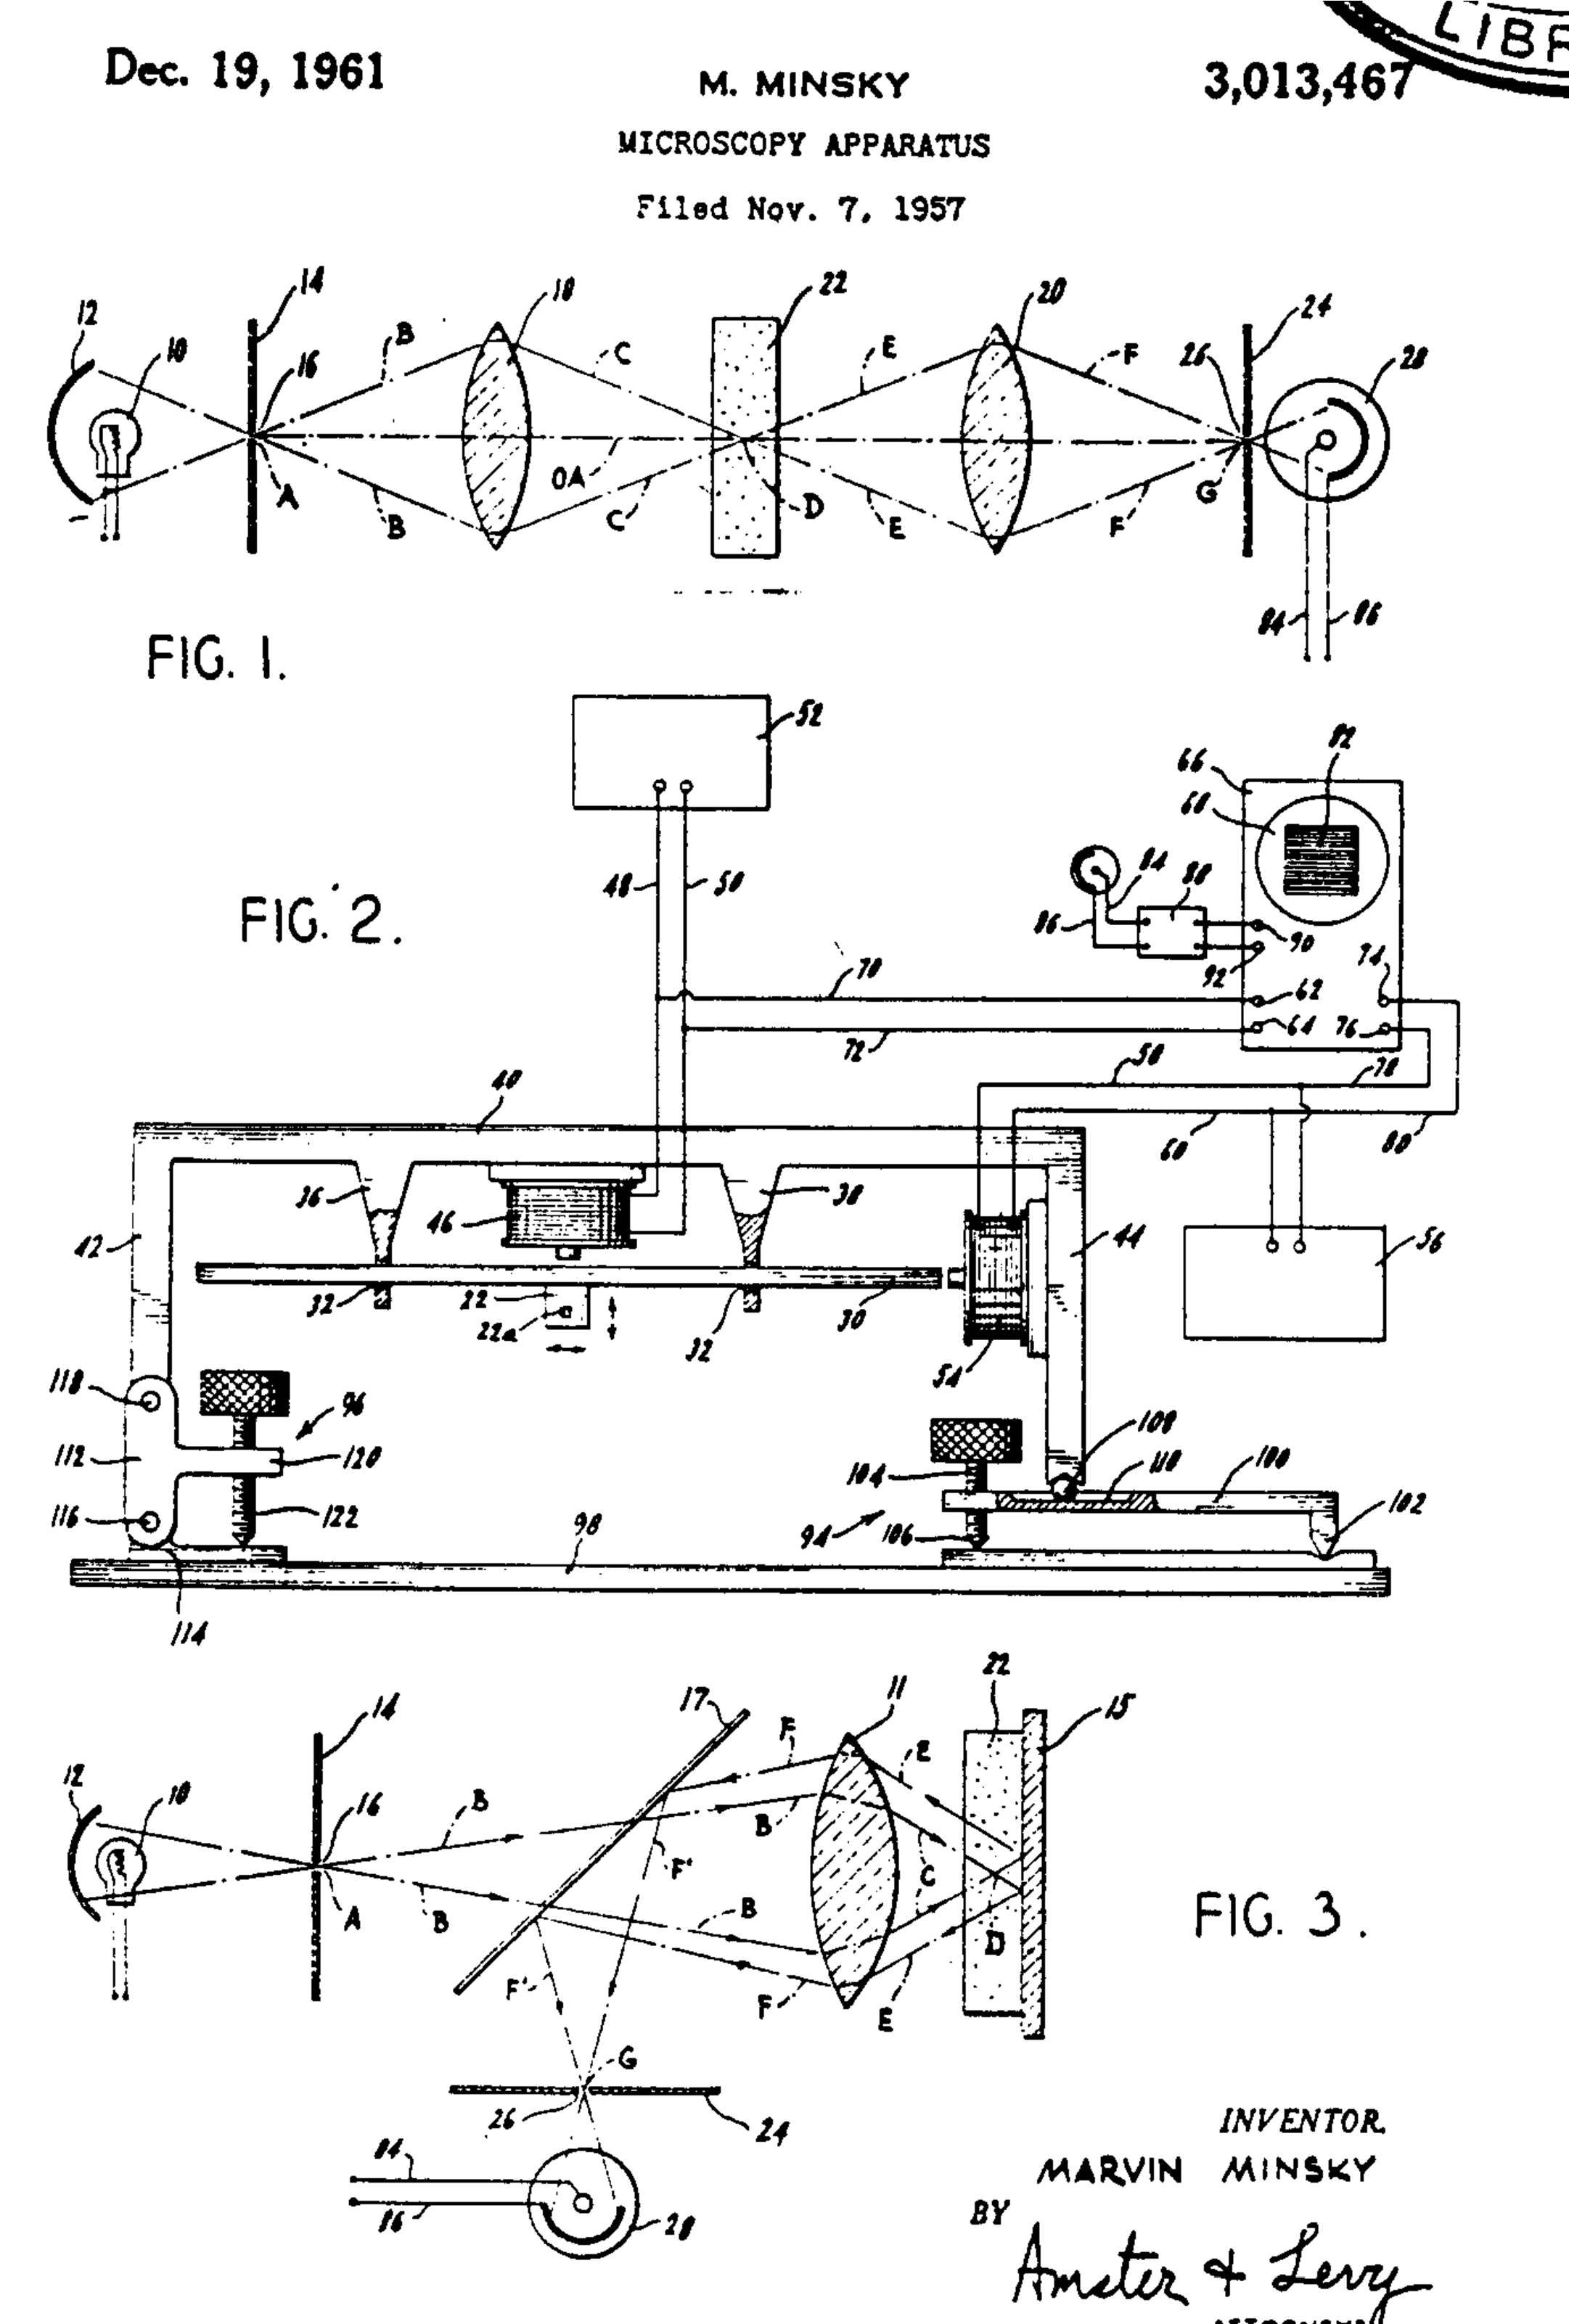
\includegraphics[width=.3\linewidth]{confocal_stuff/confocalpatent}
	\caption[Minsky Patent Diagram]{Also placeholder. I think my plan is to break this into chunks, though it almost deserves it's own appendix.}
	\label{fig:confocalpatent}
\end{figure}
\cite{patent:3013467} 

\subsection{Preparing a Fluorescent Bead Solution}
Make sure to also note that the solution should be wrapped to avoid light exposure and to keep them in the refrigerator. \todo[inline, color=yellow]{I think the actual borate buffer recipe might belong in an appendix}

\section{Image Analysis}
In the following section, we will step through the process of analyzing a single sphere. Recall that in order to determine the surface stress and adhesion energy, we must fit a line to a collection of spheres ranging in size.  
\todo[inline,color=yellow]{Insert raw data file....currently it's in chapter 4. It should be in here instead}

\subsection{Particle Location}
To turn a raw image file (saved as a .ome.tif) into usable data, we use sophisticated MATLAB program to locate each fluorescent bead. Plotted for the sphere in Figure \ref{fig:190215g91glasssphere011surface}
\begin{figure}[h!]
	\centering
	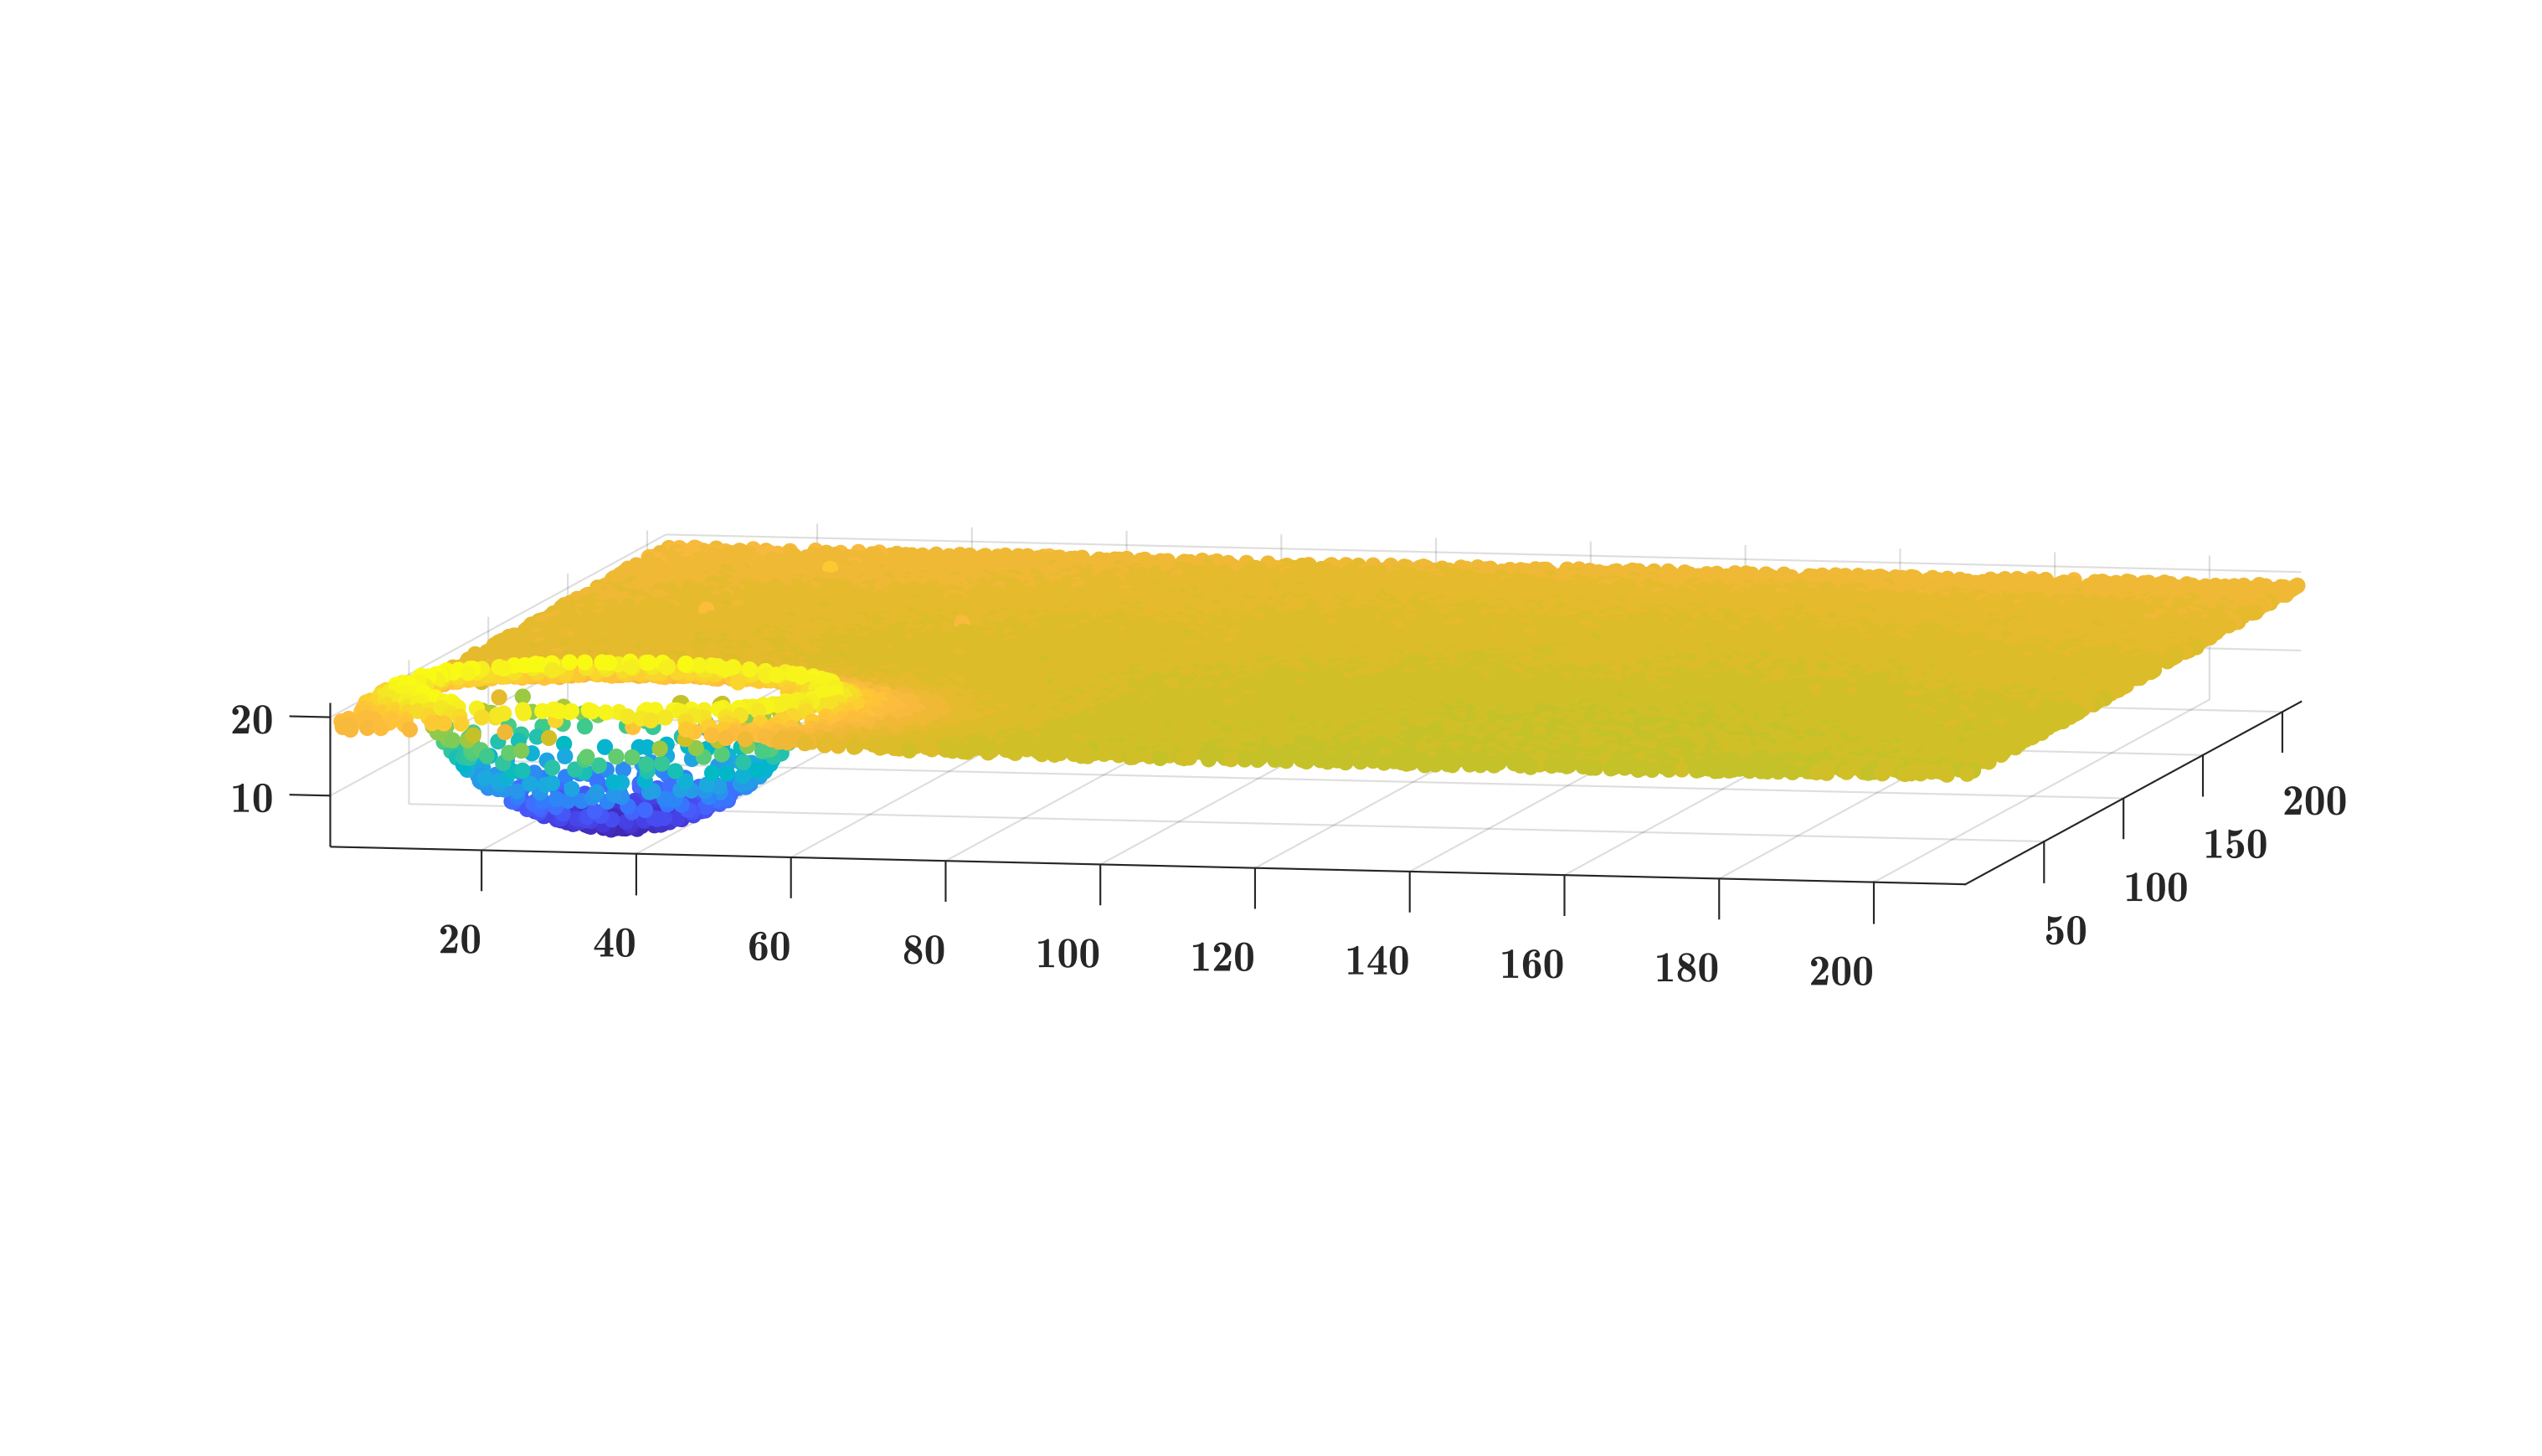
\includegraphics[width=\linewidth]{Chapters/Figures/sphere011_ia/particle_located_normalized}
	\caption[Particle Located: Normalized-Axes]{}
	\label{fig:particlelocatednormalized}
\end{figure}
\begin{figure}[h!]
	\centering
	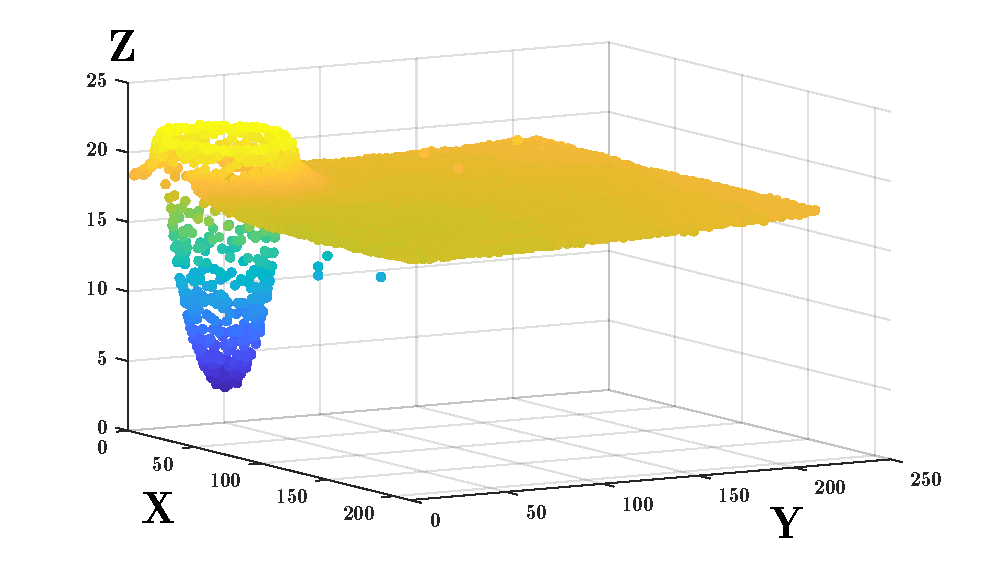
\includegraphics[width=\linewidth]{Chapters/Figures/sphere011_ia/particle_located_stretched}
	\caption[Particle Located: Stretched-Axes]{}
	\label{fig:particlelocatedstretched}
\end{figure}




\begin{figure}
	\centering
	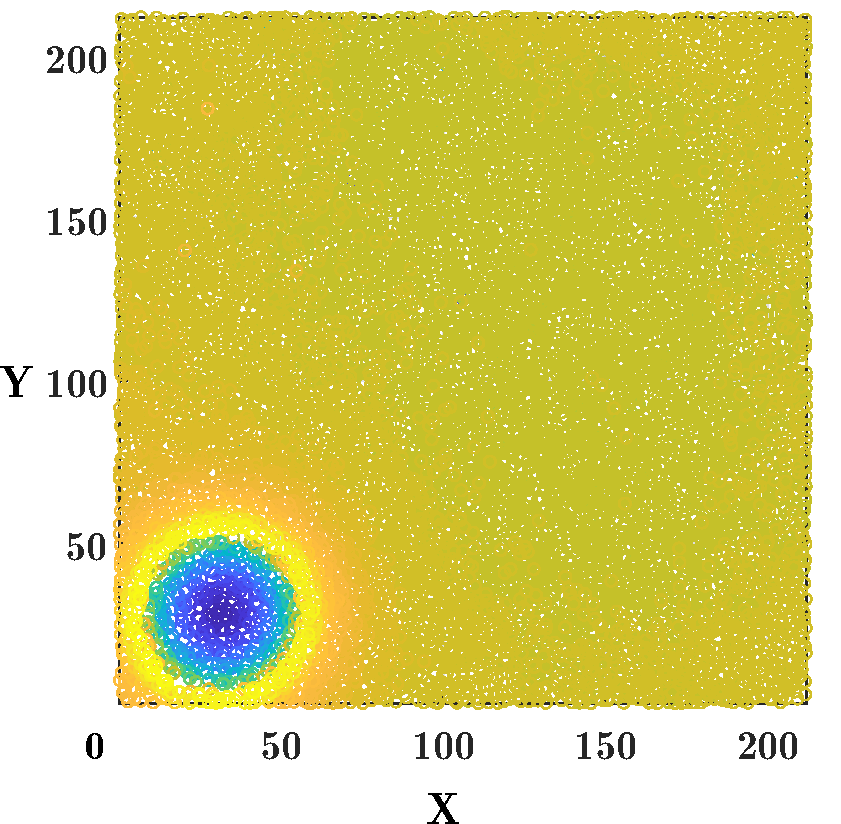
\includegraphics[width=\linewidth]{Chapters/Figures/sphere011_ia/particle_located_top_view}
	\caption[Particle Located: Top View]{}
	\label{fig:particlelocatedtopview}
\end{figure}
\begin{figure}
	\centering
	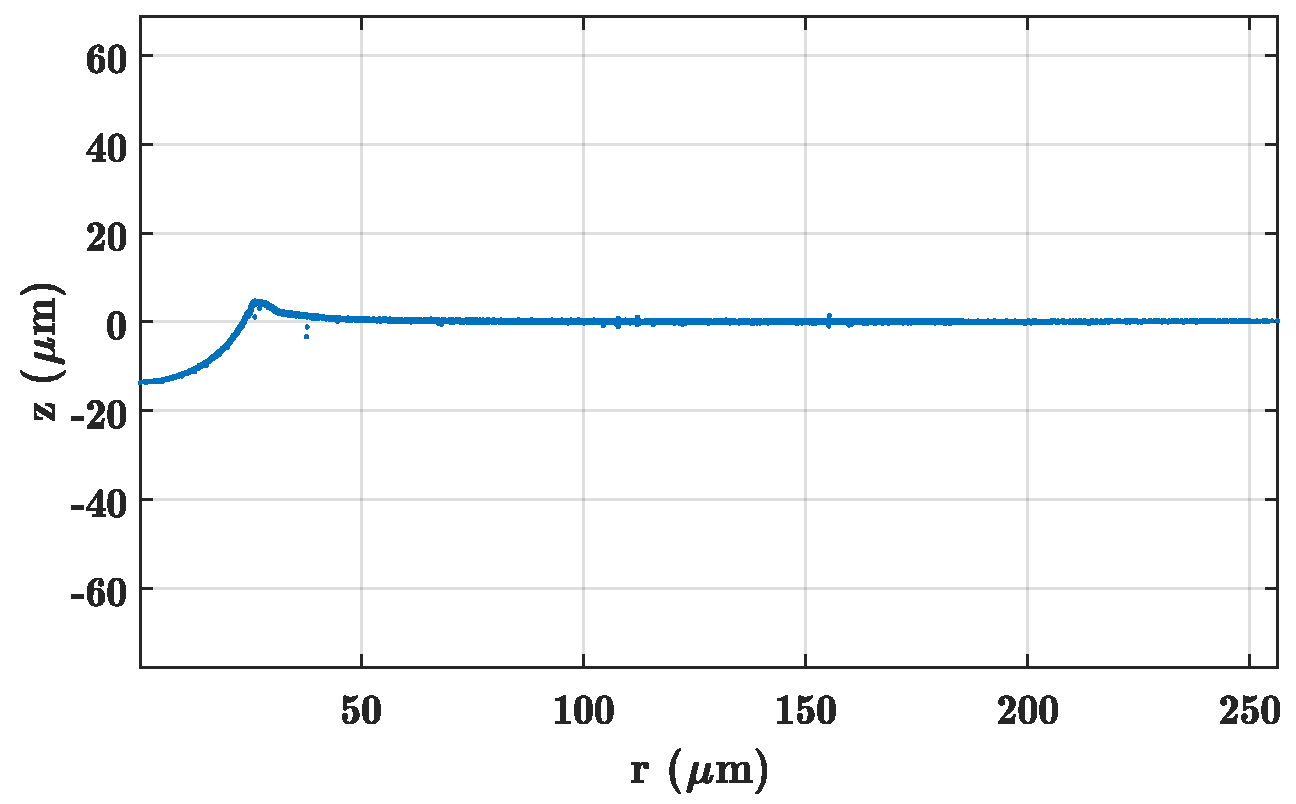
\includegraphics[width=\linewidth]{Chapters/Figures/sphere011_ia/side_collapsed}
	\caption[Collapsed Side Profile]{}
	\label{fig:sidecollapsed}
\end{figure}
\begin{figure}
	\centering
	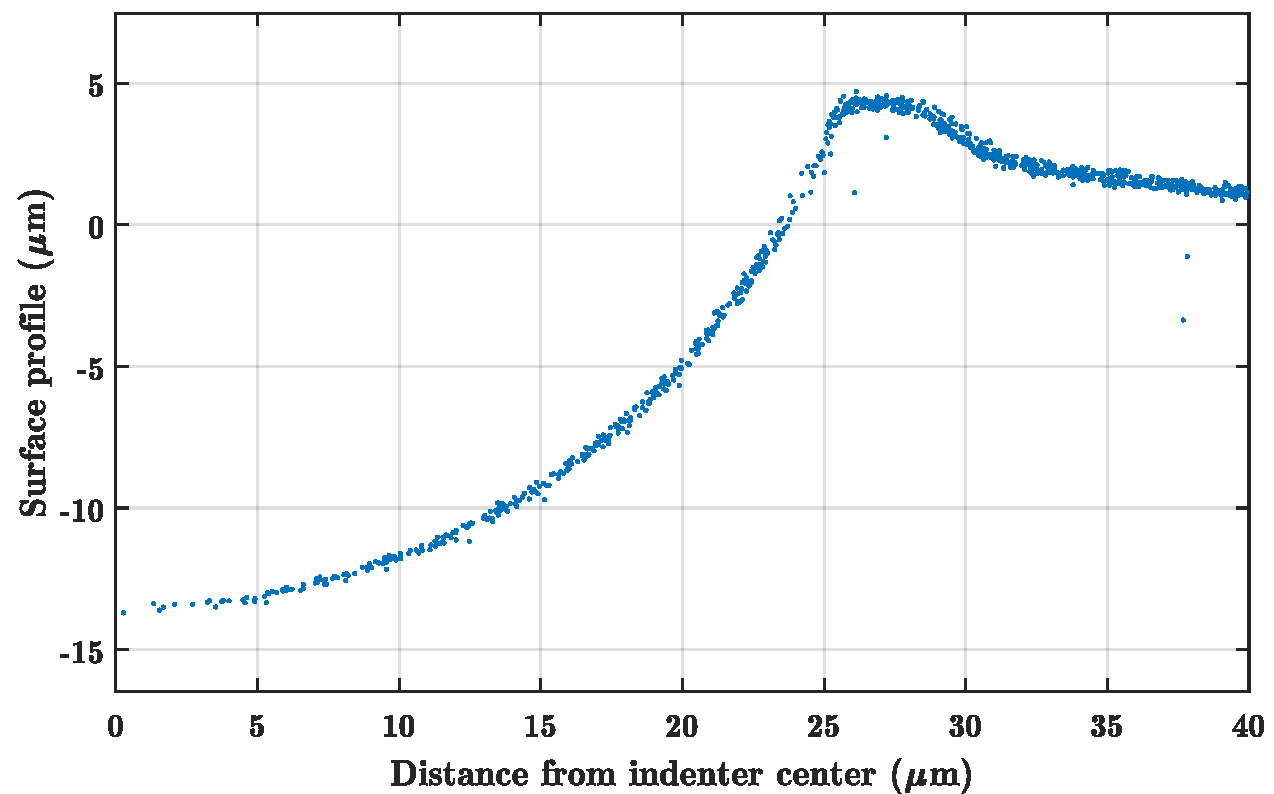
\includegraphics[width=\linewidth]{Chapters/Figures/sphere011_ia/side_collapsed_zoomed}
	\caption[Collapsed Side Profile: Zoomed]{}
	\label{fig:sidecollapsedzoomed}
\end{figure}

\begin{figure}
	\centering
	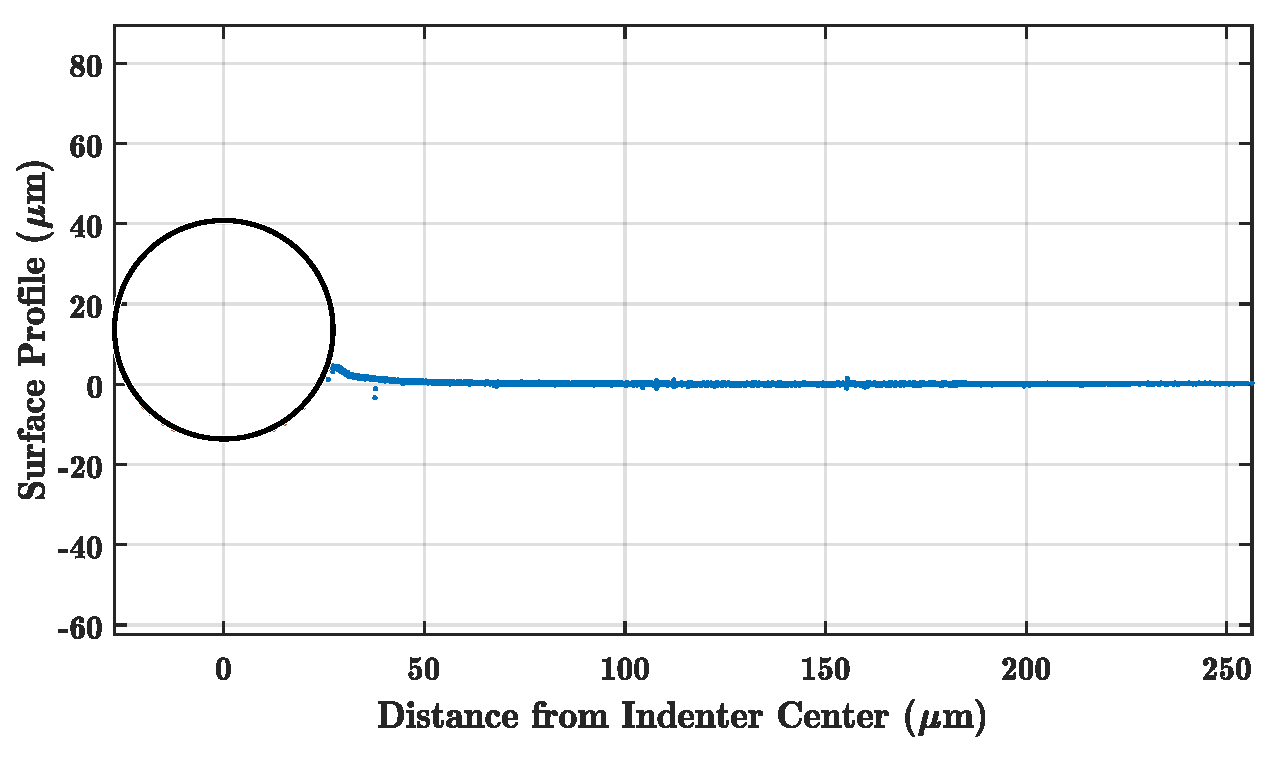
\includegraphics[width=\linewidth]{Chapters/Figures/sphere011_ia/circle_fit}
	\caption[Circle Fit]{Notice how the surface plane is completely flat and centered at a depth of 0.}
	\label{fig:circlefit}
\end{figure}
\begin{figure}
	\centering
	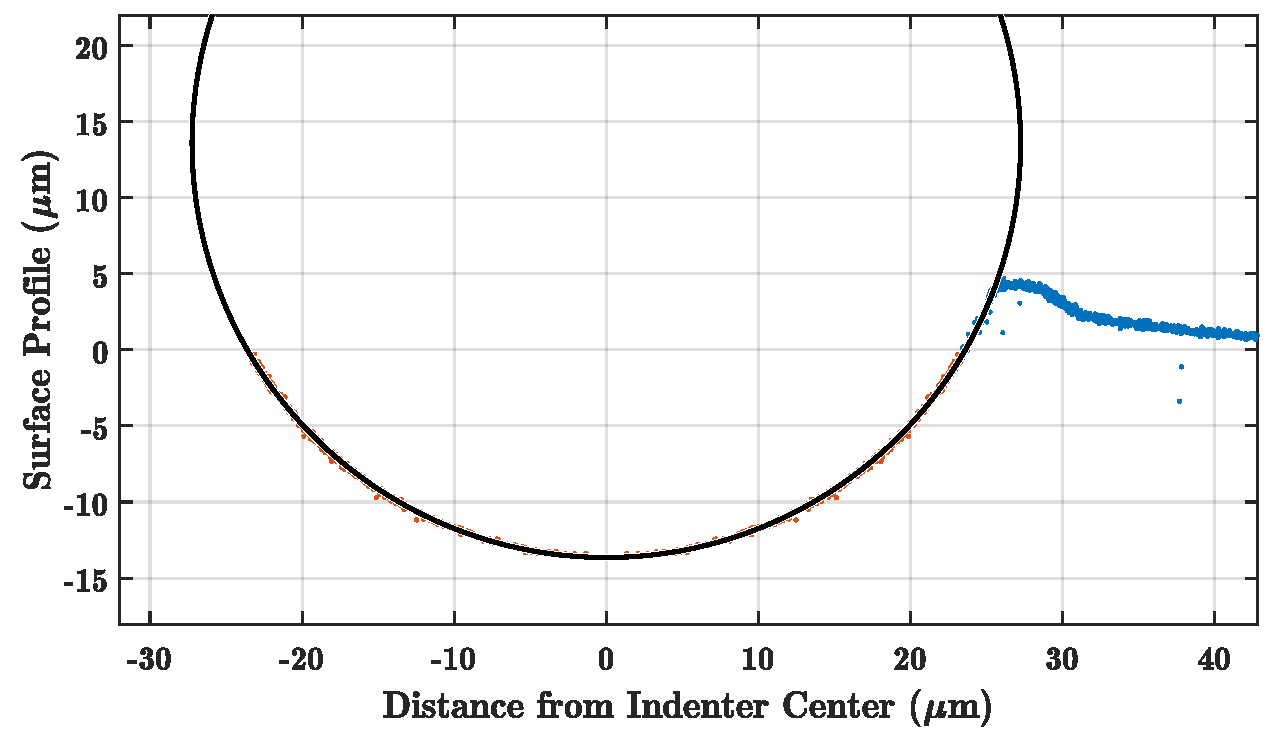
\includegraphics[width=\linewidth]{Chapters/Figures/sphere011_ia/circle_fit_zoomed}
	\caption[Circle Fit Zoomed]{The orange dots are the data points being used to fit the circle. Notice how the sphere fits nicely in the indentation all the way up to the cusp, past the points being used for the fit.}
	\label{fig:circlefitzoomed}
\end{figure}
\begin{figure}
	\centering
	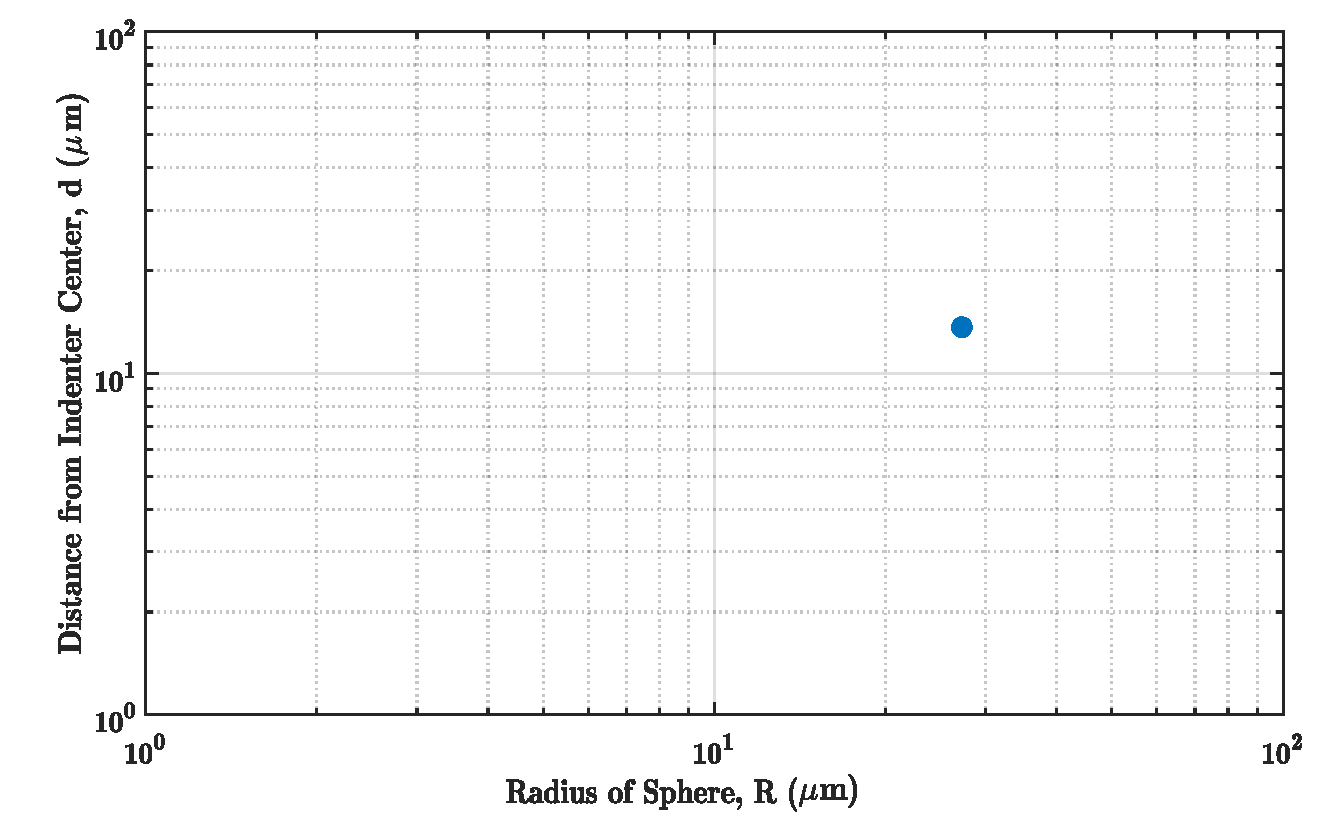
\includegraphics[width=\linewidth]{Chapters/Figures/sphere011_ia/single_d_vs_r}
	\caption[D vs R plot]{}
	\label{fig:singledvsr}
\end{figure}
